% ============================================================
% Neural Demand — Habit Advantage Table (auto-generated)
% N_RUNS = 2
% ============================================================

\begin{table}[htbp]
  \centering
  \caption{Habit-State Augmentation Advantage --- Simulation  (2 runs; mean $\pm$ SE)}
  \label{tab:sim_habit_advantage}
  \begin{threeparttable}
  \begin{tabular}{lcccc}
    \toprule
    \textbf{Model} & \textbf{RMSE} & \textbf{KL Div.}    & \textbf{RMSE Red.\ (\%)} & \textbf{CV} \\
    \midrule
    LA-AIDS & $0.04338 \pm 0.00113$ & $0.00793 \pm 0.00032$ & 0.0\% & {---} \\
    Logit-IV & $0.04476 \pm 0.00093$ & $0.01855 \pm 0.00033$ & -3.2\% & {---} \\
    QUAIDS & $0.04304 \pm 0.00137$ & $0.00780 \pm 0.00036$ & 0.8\% & {---} \\
    Series Estm. & $0.03974 \pm 0.00229$ & $0.00650 \pm 0.00063$ & 8.5\% & {---} \\
    Linear Demand (Shared) & $0.14414 \pm 0.00273$ & $0.10409 \pm 0.00588$ & -232.3\% & {---} \\
    Linear Demand (GoodSpec) & $0.14485 \pm 0.00330$ & $0.10503 \pm 0.00665$ & -234.0\% & {---} \\
    Linear Demand (Orth) & $0.04531 \pm 0.00093$ & $0.00866 \pm 0.00026$ & -4.5\% & {---} \\
    Neural Demand (static) & $0.04176 \pm 0.00143$ & $0.00735 \pm 0.00035$ & 3.7\% & {---} \\
    Neural Demand (habit) & $0.02328 \pm 0.00125$ & $0.00246 \pm 0.00031$ & 46.4\% & {---} \\
    Neural Demand (CF) & $0.04223 \pm 0.00090$ & $0.00751 \pm 0.00020$ & 2.6\% & {---} \\
    Neural Demand (habit, CF) & $0.02639 \pm 0.00088$ & $0.00319 \pm 0.00028$ & 39.2\% & {---} \\
    \bottomrule
  \end{tabular}
  \begin{tablenotes}\small
    \item True DGP: \texttt{HabitFormationConsumer} with    $\delta_{true}=0.7$.    $\hat{\delta} = 0.650 \pm    0.050$ (mean $\pm$ SE over 2 runs).    True $\delta$ in identified set: 100\% of seeds.
  \end{tablenotes}
  \end{threeparttable}
\end{table}

% ============================================================
% Figure environments
% ============================================================

\begin{figure}[htbp]
  \centering
  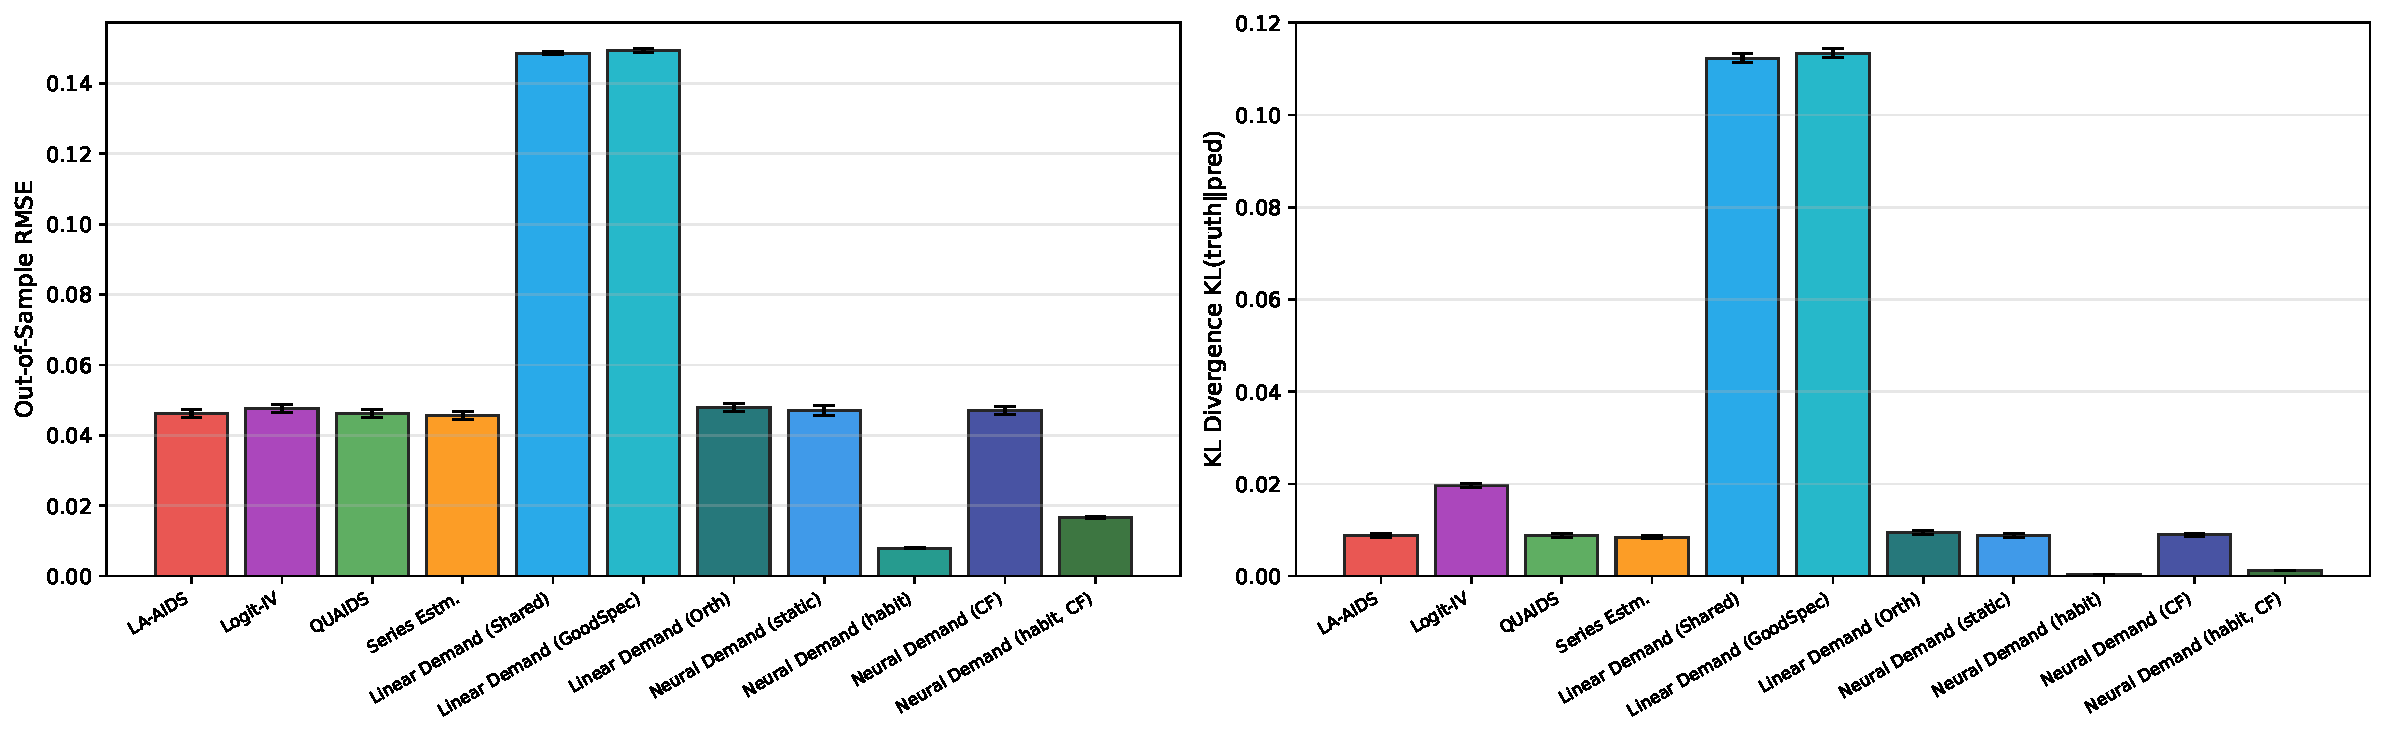
\includegraphics[width=0.85\linewidth]{results/neural_demand/simulations/figures/fig_habit_advantage.pdf}
  \caption{Habit-State Augmentation Advantage.  RMSE (left) and KL divergence (right) on post-shock test data.  Shaded bands = ±1 SE across runs.}
  \label{fig:sim_habit_advantage}
\end{figure}

\begin{figure}[htbp]
  \centering
  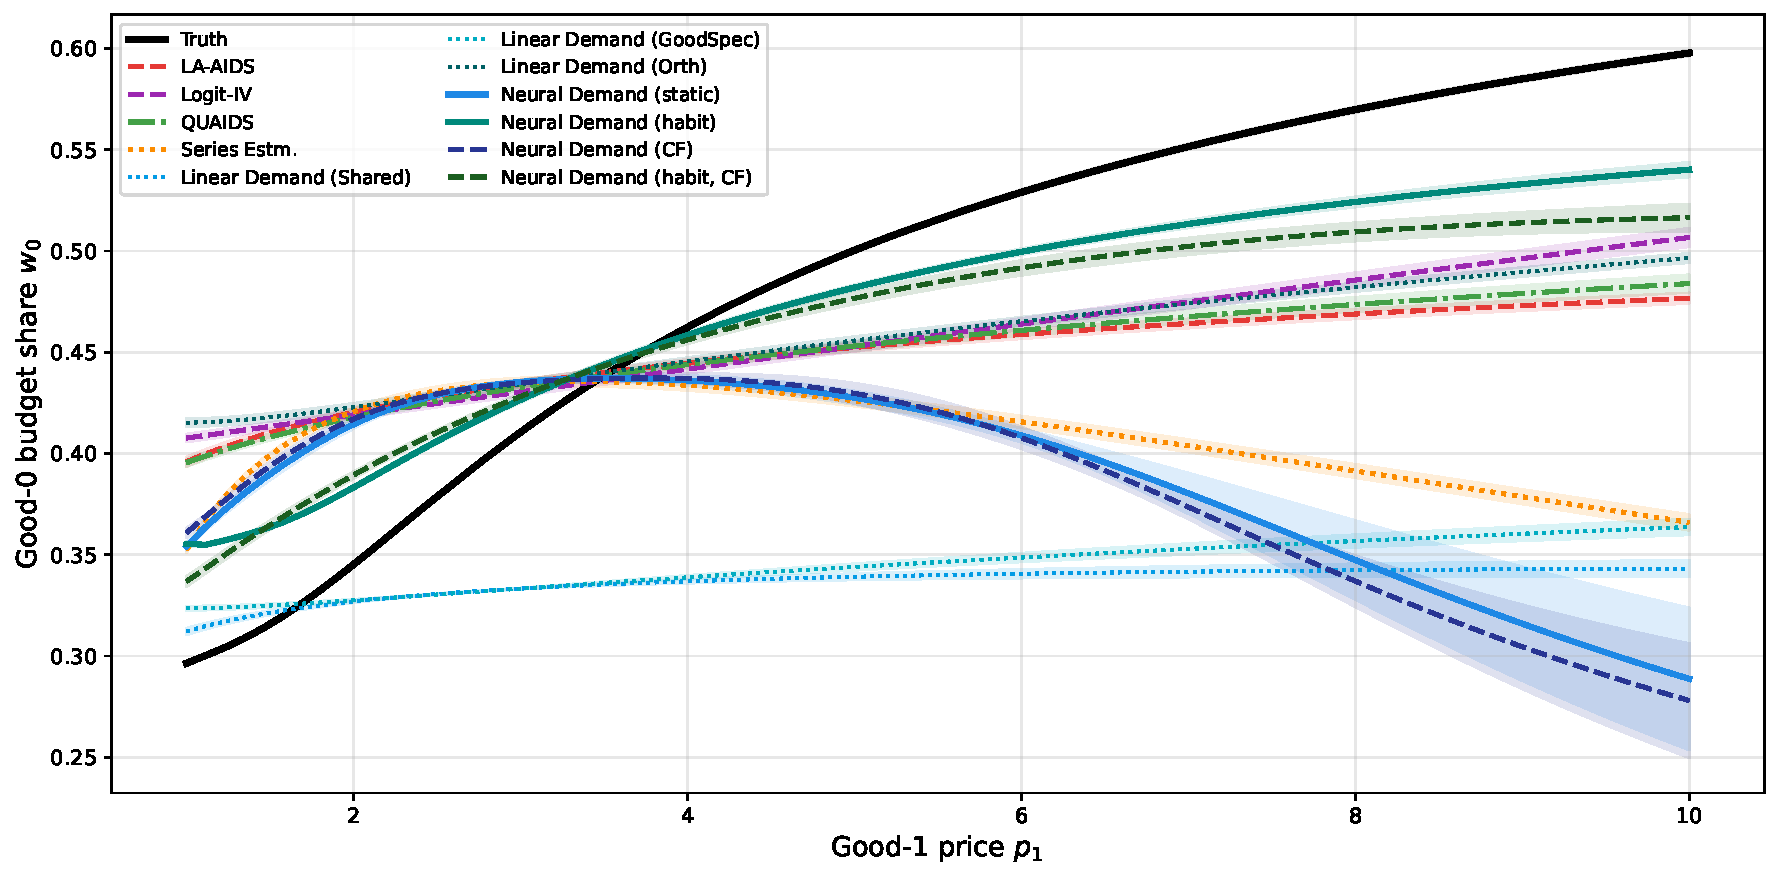
\includegraphics[width=0.85\linewidth]{results/neural_demand/simulations/figures/fig_habit_demand_curves.pdf}
  \caption{Demand Curves under Habit DGP.  Good-0 budget share as a function of good-1 price.  Habit-augmented model best tracks the true curve.}
  \label{fig:sim_habit_curves}
\end{figure}

\begin{figure}[htbp]
  \centering
  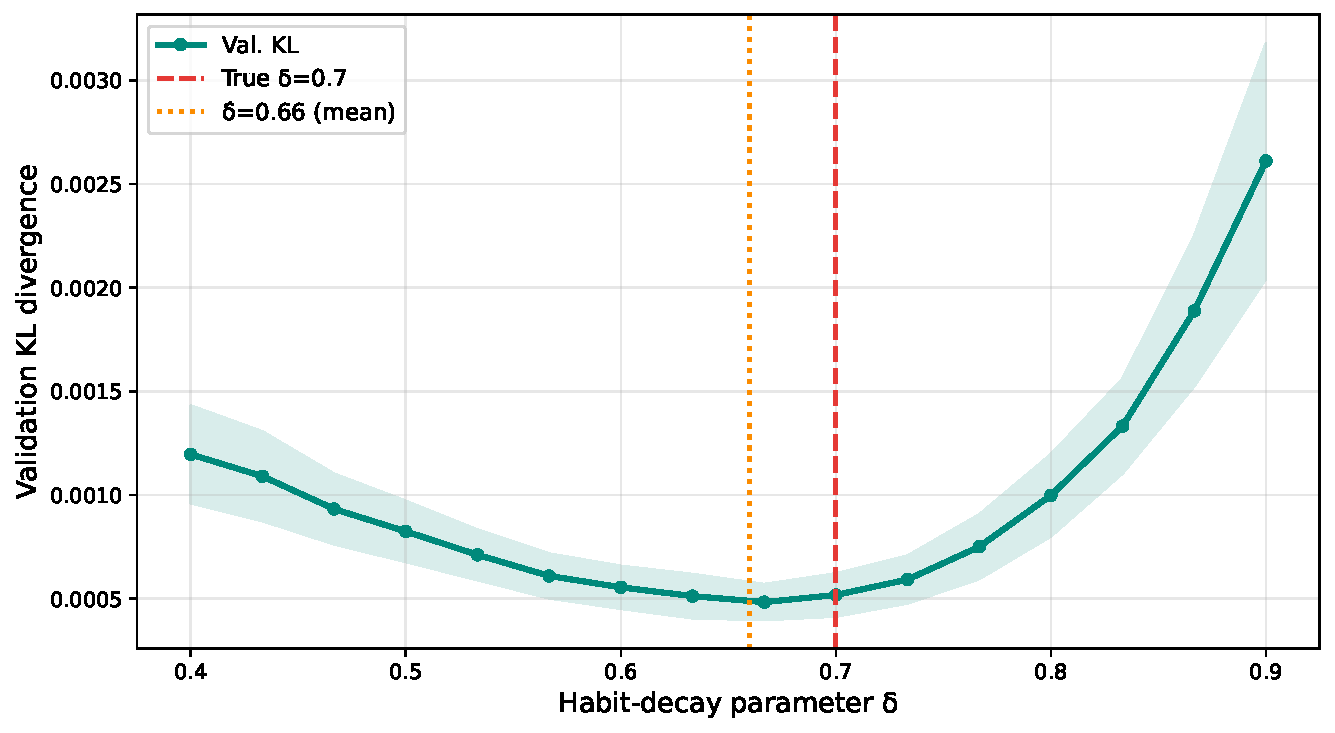
\includegraphics[width=0.85\linewidth]{results/neural_demand/simulations/figures/fig_habit_profile_kl.pdf}
  \caption{Profile KL criterion for $\delta$ identification.  The flat region spans the identified set.}
  \label{fig:sim_habit_profile_kl}
\end{figure}
